\section{Simulationsbeispiel}
Die vorgestellten Methoden zur lokalen Stabilitätsanalyse eines Netzwerks werden, in diesem Abschnitt auf ein Beispiel angewendet. Bisher wurden nur dynamische Systeme mit kontinuierlichen Variablen betrachtet. Die zugrunde liegende Theorie lässt sich auch auf diskrete Systeme anwenden. Dabei ist die Dynamik nicht durch ein Differentialgleichungssystem gegeben, sondern durch eine Iterationsvorschrift. Das hier betrachtete Netzwerk  folgt der Dynamik in (\ref{eq:bspdyn})\cite{pecora2014}.
\begin{align}
\label{eq:bspdyn}
	x_i^{t+1}&=\left[\beta\mathcal{I}(x_i^t)+\sigma \sum_j^N A_{ij}\mathcal{I}(x_j^t)+\delta\right] \text{mod}\quad 2\pi
	\\\notag & \beta,\sigma \text{ Kopplungsparameter}
	\\\notag  & \delta \text{ Offset}
	\\\notag &\mathcal{I}(x)=\frac{1-Cos(x)}{2}
\end{align}
Die betrachteten Netzwerke sind symmetrisch und bestehen aus $N=11$ Knoten  (Abb. \ref{fig:cluster}). Die verwendeten Kopplungsmatrizen sind Pecora et al.entnommen und in Abb. \ref{fig:abmat} dargestellt (siehe auch Anhang)\cite{pecora2014}. Für diese Netwerke ergibt die Suche nach Automorphismen der zugrundeliegenden Graphen mit \textit{Nauty} 0, 32 bzw. 5760 Symmetrien und 11 (triviale, nur aus einem Knoten bestehende), 5 bzw. 3 Cluster (Tab. \ref{tab:netzwerke}).Zur Berechnung der Ljaponow-Exponenten für die verschiedenen Cluster wurde eine Basistransformation (siehe \ref{stabilitaet}) mit den im Anhang dargestellten Transformationsmatrizen vorgenommen \cite{pecora2014,sagenotebook}.

Für Netzwerk 1 erübrigt sich aufgrund des Fehlens von Clustern die Stabilitätsanalyse.\\


\begin{figure}
	 \centering
	 \subfloat[Netzwerk 1]{
	 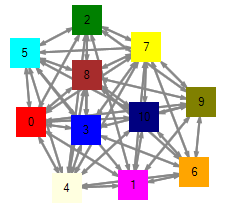
\includegraphics[width=0.25\textwidth]{abb/misc/cluster1.png}
	 }
	 \subfloat[Netzwerk 2]{
	 	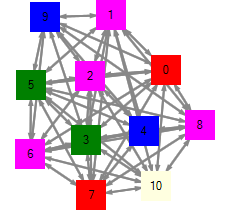
\includegraphics[width=0.25\textwidth]{abb/misc/cluster2.png}
	 }
	 \subfloat[Netzwerk 3]{
	 	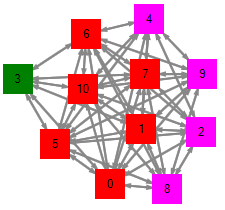
\includegraphics[width=0.25\textwidth]{abb/misc/cluster3.png}
	 }
	 \caption[In der Simulation verwendete Netzwerke]{Die drei verwendeten Netzwerke. Die Knoten eines Cluster sind in der gleichen Farbe eingefärbt.}
	 \label{fig:cluster}
	 
\end{figure}

\begin{figure}
	\centering
	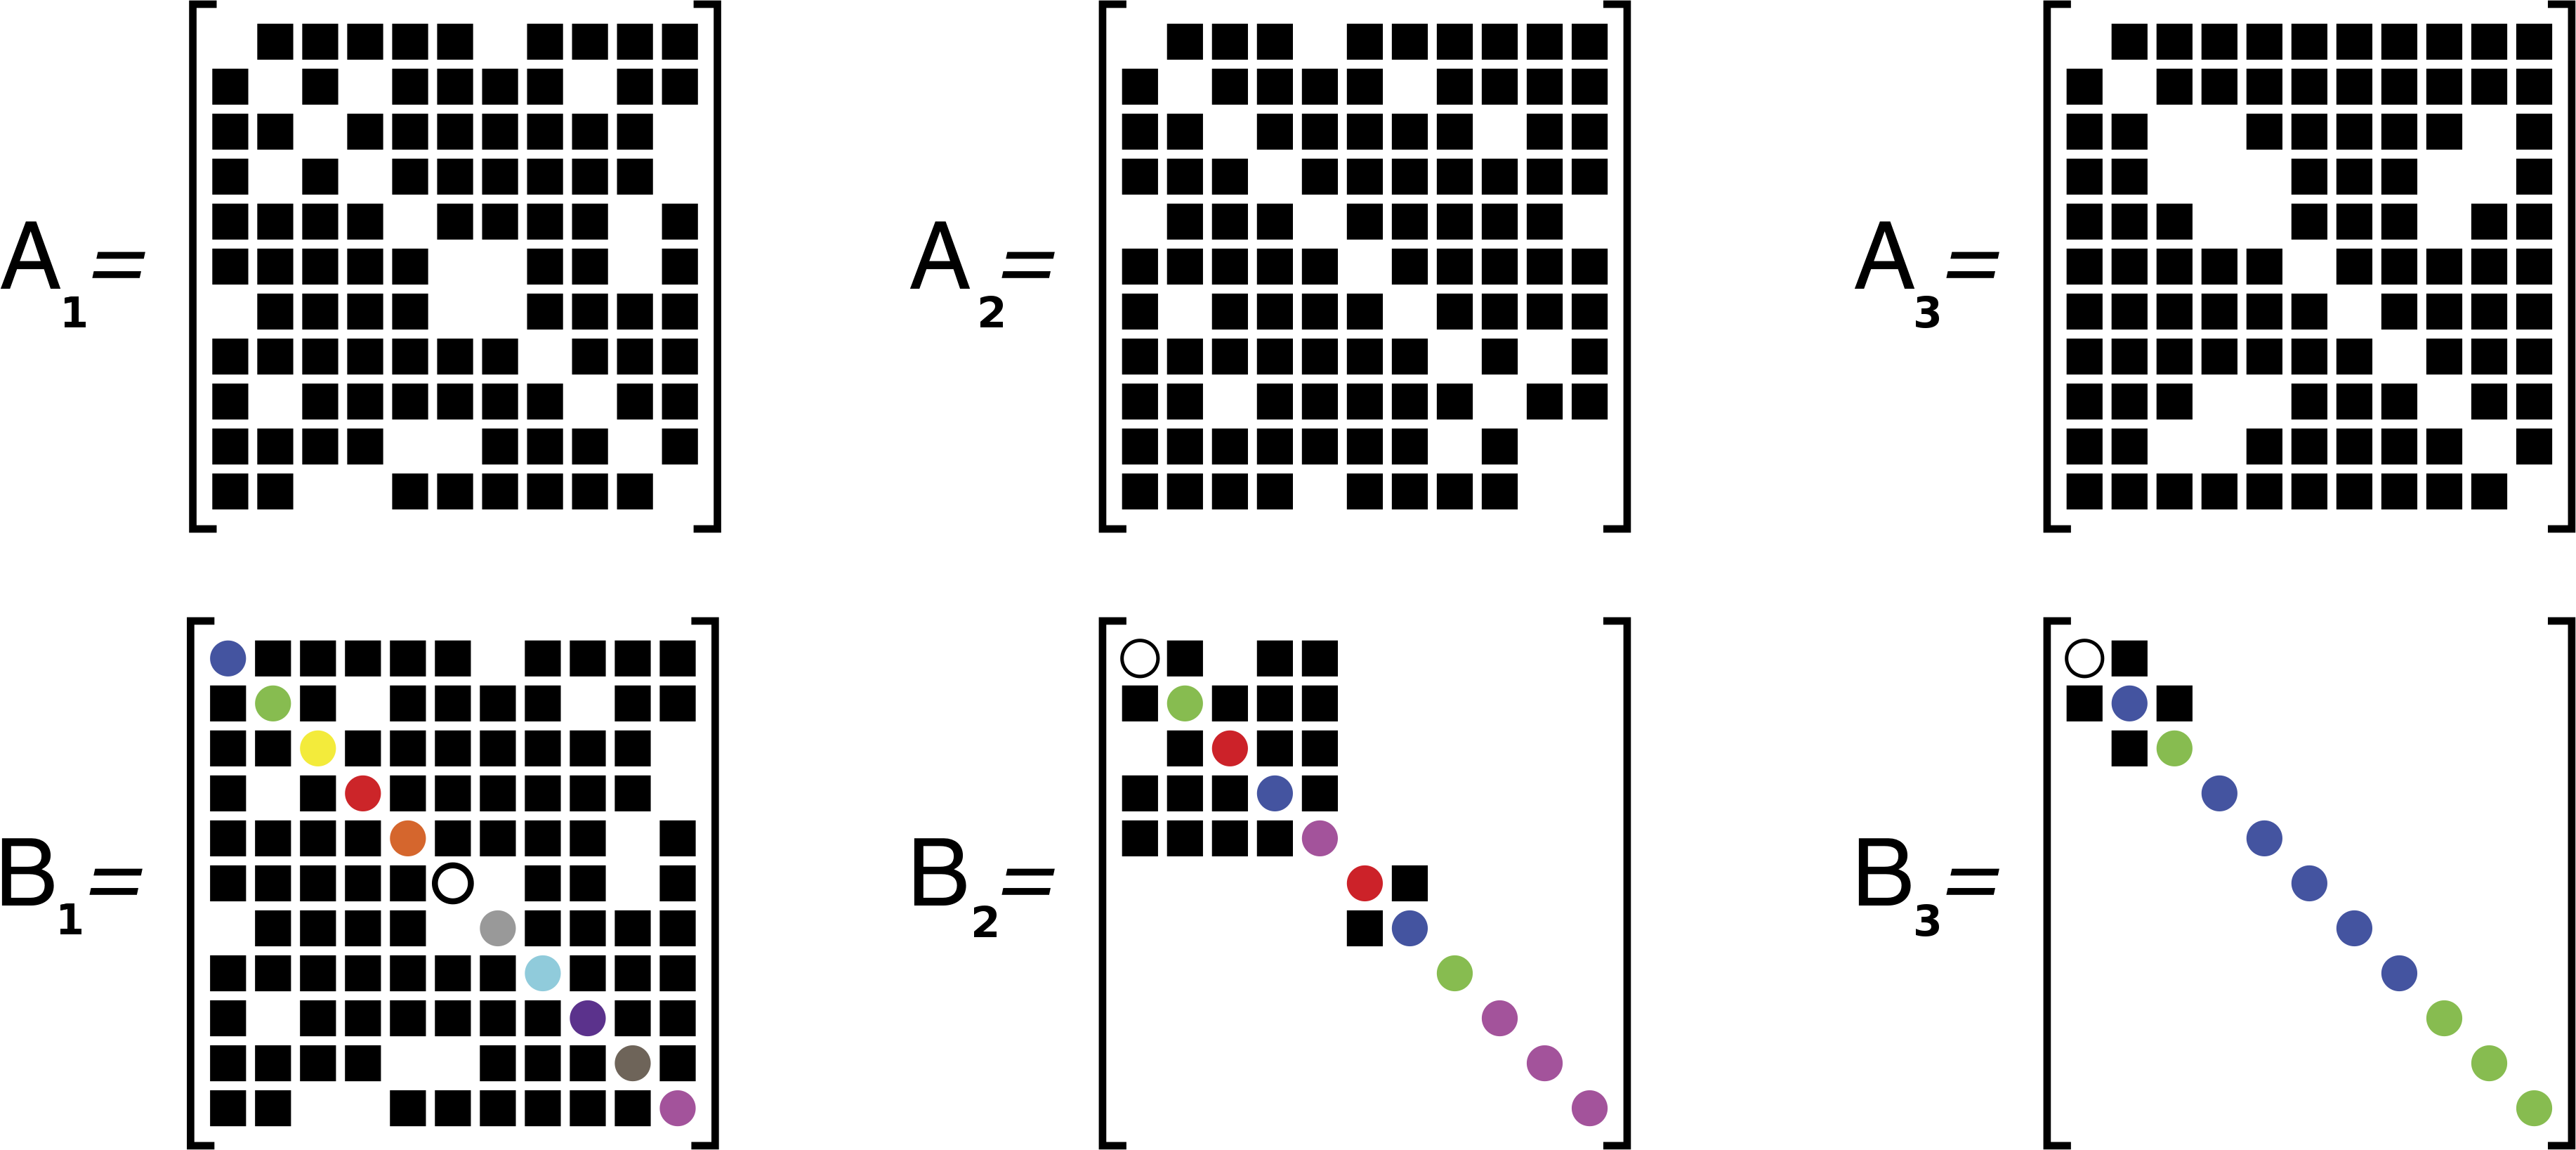
\includegraphics[width=0.75\textwidth]{abb/misc/ABMat.png}
	\caption{Kopplungsmatrizen $\boldsymbol{A}$ der in Abb. \ref{fig:cluster} dargestellten Netwerke sowie die transformierte Kopplungsmatrizen $\boldsymbol{B}$ in der die Zeilen nach den zugehörigen Clustern markiert sind\cite{pecora2014}.}
\label{fig:abmat}
\end{figure}

\begin{table}[]
	\begin{center}
		\caption{Symmetrien und Cluster der betrachteten Netzwerke}
		\label{tab:netzwerke} 
		
		\begin{tabular}{lll}
			Netzwerk & Symmetrien & Cluster                           \\
			\hline
			1        & 0          & 11 triviale Cluster               \\
			2        & 32         & (1,8) (2,3,7,9) (4,6) (5,10) (11) \\
			3        & 5760       & (1,2,6,7,8,11) (3,5,9,10) (4) \\  
			\hline
		\end{tabular}
	\end{center}
\end{table}
\begin{figure}
	\centering
	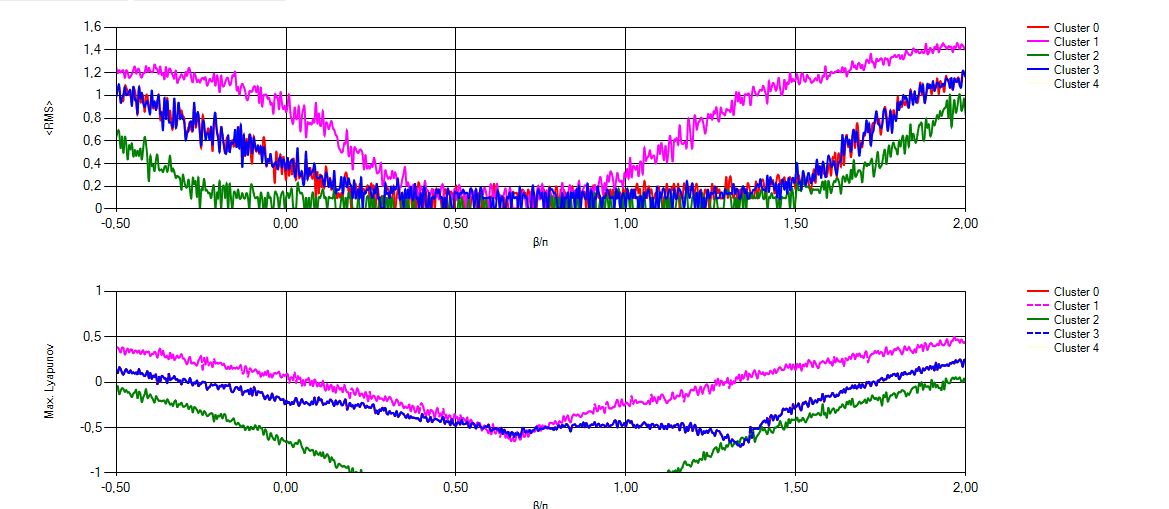
\includegraphics[width=1.0\textwidth]{abb/misc/ljapResult.png}
	\caption{Ergebnisse der Simulation. Die obere Grafik zeigt die mittlere quadratische Abweichung vom Mittelwert für das jeweilige Cluster. Im unteren Bild ist der maximale Ljapunow-Exponent für die Cluster über $\beta$ aufgetragen. Nach einer Transienten von 200 Zeitschritten wurden die mittleren Abweichungen über 1000 weitere Schritte gemittelt. $\beta$ nimmt im Intervall $[-\frac{1}{2}\pi,2\pi]$ 400 Werte an.}
	\label{fig:ljapResult}
\end{figure}
Abb. \ref{fig:ljapResult} zeigt exemplarisch die Simulationsergebnisse für das zweite Netzwerk bei Variation des Parameters $\beta$. Dabei beschreibt RMS die mittlere quadratische Abweichung vom Mittelwert für ein Cluster, also ein Maß für die Asynchronizität eines Clusters. Die Anfangswerte $x_i^0$ sind gaußverteilt um $\pi$ mit einer Standardabweichung von 0,01$\pi$ gewählt, also zunächst asynchron. Ein geringes Rauschen von 0,002 ist in jedem Iterationsschritt eingefügt, sodass die Synchronisation zusätzlich gestört wird.
Die RMS-Abweichung von der Synchronisation geht gegen Null, sobald die MSF negativ wird. Dies stimmt mit den Überlegungen aus \ref{stabilitaet} überein, da die Bahnkurven sich für lange Zeiten wieder annähern, also synchron laufen.
Alle Cluster außer 0 (Rot) und 3 (Blau) weisen eine isolierte Synchronisation auf. Die Synchronisation innerhalb eines Clusters ist unabhängig vom Zustand der anderen. Das blaue und rote Cluster hingegen verlieren (bzw. erreichen) die Synchronizität gemeinsam, sind also interwinded Cluster. Dies wird durch den identischen Verlauf der MSF deutlich.\\
Zusätzlich zur Variation über $\beta$ kann der größte Ljapunow-Exponent auch für beliebige $(\beta,\sigma)$-Paare berechnet werden.
\begin{figure}[h]
	\centering
	\subfloat[Cluster 0]{
		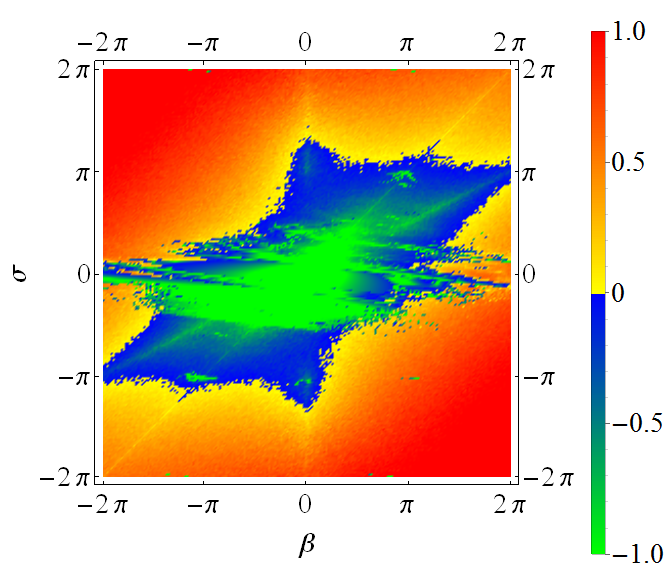
\includegraphics[width=0.45\textwidth]{abb/misc/Plot2D_Cluster0.png}
	}
	\subfloat[Cluster 1]{
		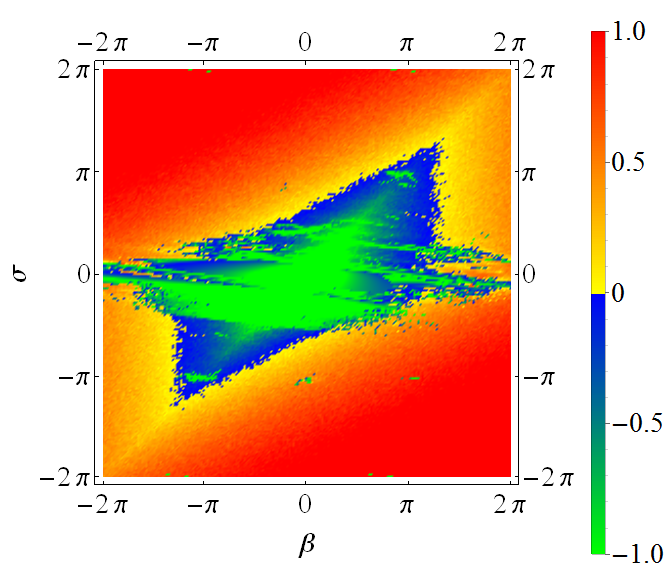
\includegraphics[width=0.45\textwidth]{abb/misc/Plot2D_Cluster1.png}
	}\\
	\subfloat[Cluster 2]{
		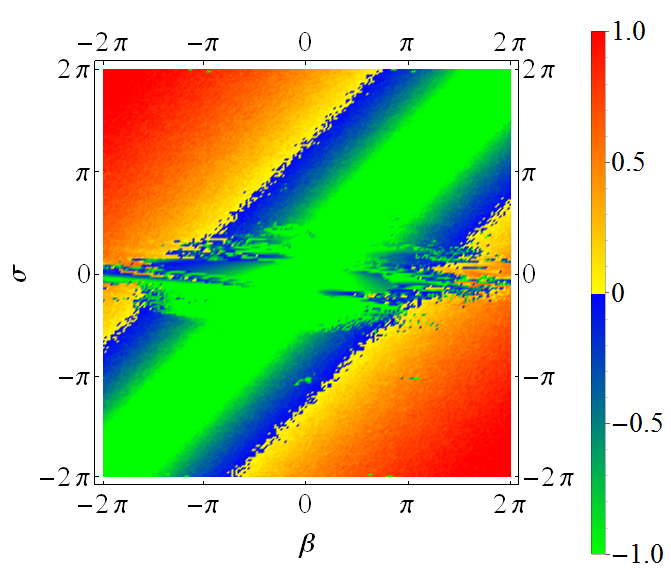
\includegraphics[width=0.45\textwidth]{abb/misc/Plot2D_Cluster2.png}
	}
	\subfloat[Cluster 3]{
		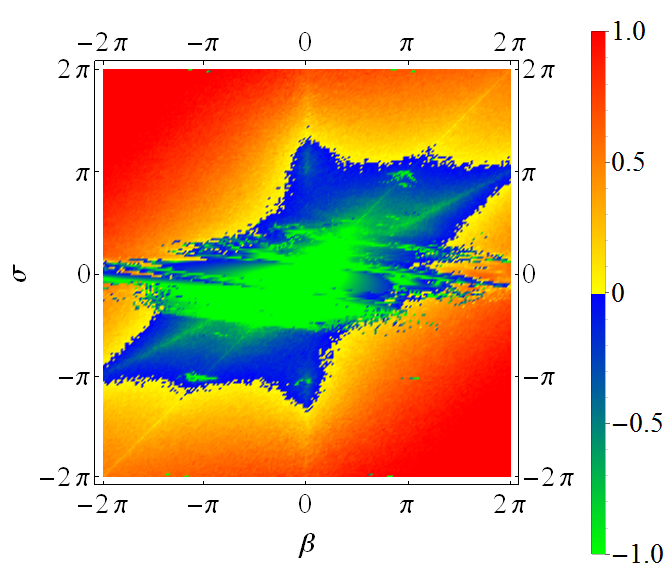
\includegraphics[width=0.45\textwidth]{abb/misc/Plot2D_Cluster3.png}
	}
	\caption{Größter Ljapunow-Exponent für die unterschiedlichen Cluster aufgetragen über $\beta$ und $\sigma$. Die blau-grünen Bereiche sind stabil und die gelb-roten instabil. Nach einer Transienten von 100 Zeitschritten wurden 500 weitere Schritte für die Berechnung verwendet. $\beta$ und $\sigma$ nehmen jeweils 200 Werte im Intervall $[-2\pi,2\pi]$ an.}
	\label{fig:2dplots}	
\end{figure}
Abb. \ref{fig:2dplots} zeigt die größten Ljapunow-Exponenten für die verschiedenen Cluster aufgetragen über $\beta$ und $\sigma$. Mithilfe dieser Darstellung kann direkt abgelesen werden, für welche Parameterpaare das synchrone Verhalten der einzelnen Cluster stabil oder instabil ist. Man erkennt auch hier wieder, dass Cluster 0 und Cluster 3 interwinded Cluster sind, da sich die Stabilität gleich verhält. Ist $\sigma$ nahe 0, so sind die Knoten des Netzwerks näherungsweise ungekoppelt und die Dynamik für jeden Knoten (unabhängig von seiner Clusterzugehörigkeit) gleich. Die Ljapunow-Exponenten in diesem Bereich sind folglich in allen Clustern gleich und in Abb. \ref{fig:sigma0} dargestellt. 
\begin{figure}
	\centering
	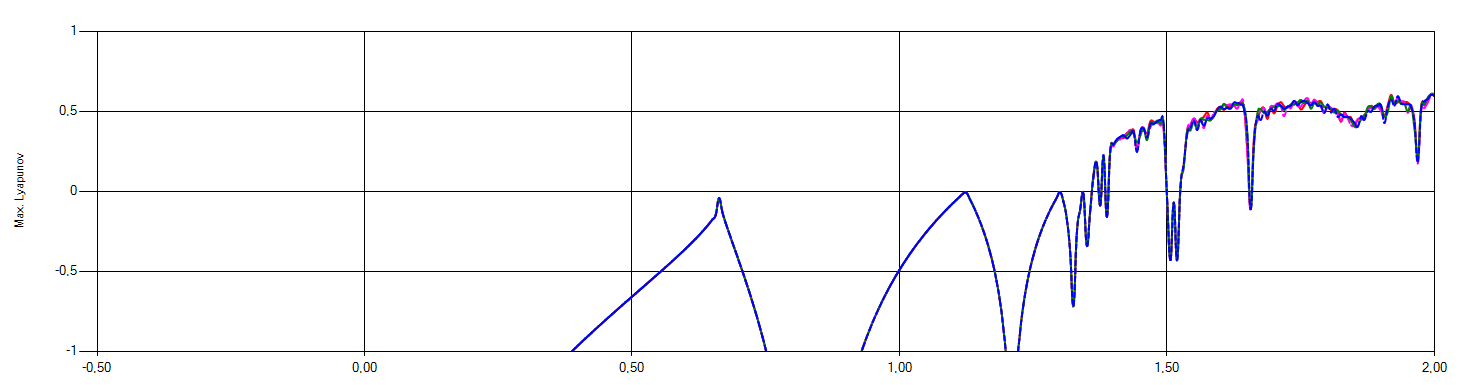
\includegraphics[width=1.0\textwidth]{abb/misc/sigma0.png}
	\caption{Ergebnisse der Simulation für $\sigma=0$. Aufgetragen ist der größte Ljapunow-Exponent für einen beliebigen Knoten/ein beliebiges Cluster über 400 $\beta$ Werte im Intervall $[-\frac{1}{2}\pi,2\pi]$.}
	\label{fig:sigma0}
\end{figure}\\
Analoge Beobachtungen können bei dem dritten Netzwerk gemacht werden. Auch hier verschwindet die Asynchronizität der Cluster bei negativer MSF (nicht dargestellt). Die Methode zur Stabilitätsuntersuchung lässt sich auch bei diesem anwenden.